\chapter{Related work}
\label{chap:rel-work}

In this chapter, we describe the background research conducted. We introduce both \acrfull{ad} and \acrfull{al} and show how they are treated in the literature. We then describe some \acrshort{al} techniques applied to different contexts.
% This chapter describes the background research conducted in literature to find state-of-the-art techniques and metrics applied to \emph{Active Learning}.

\section{Anomaly Detection}
\acrfull{ad}~\cite{ruff2021unifying} is a research field that focuses on finding anomalous observations in mostly nominal data. Its application spans multiple disciplines such as engineering, machine learning, data mining, and statistics. \acrshort{ad} has applications across different domains. Some of the domains are: cyber-security~\cite{ruff2021unifying, liao2013intrusion, xin2018machine}, robotics~\cite{mantegazza2022outlier, wellhausen2020safe}, biomedical imagery~\cite{schlegl2019f}, automatic surveillance systems~\cite{chakravarty2007anomaly}, insurance~\cite{van2016outlier} and finance~\cite{ahmed2016survey} fraud detection, and more~\cite{ruff2021unifying}.
\\
\\
Because \acrshort{ad} is applied to such a broad range of contexts, a general definition of anomaly has to be as vague as possible.
Ruff et al~\cite{ruff2021unifying} define an anomaly as: \enquote{an observation that deviates considerably
from some concept of normality}, while Chandola et al~\cite{chandola2009anomaly} define it as: \enquote{patterns in data that do not conform to expected behavior.}
Both definitions make clear that a concept of \emph{normality} has to be known and modeled to successfully perform \acrshort{ad}.
\\
\\
In this work, we apply \acrshort{ad} to corridor patrolling robots, described in~\autoref{chap:prob}. We use \acrshort{ad} techniques to images coming from the robot's camera. Currently, the state-of-the-art models for image \acrshort{ad} are \acrfull{dl} based models. Generally, these kinds of model training make use of supervised learning approaches. However, anomalous events are \emph{unexpected} and rare phenomena. For this reason, supervised learning approaches are not suitable because of the strong imbalance between the classes. Therefore in this setup unsupervised learning approaches are used. Models training uses normal data only. Their goal is to make the model learn a representation of \emph{normality}.


% In this work, we apply \acrshort{ad} to corridor patrolling robots. We thus work on images. Currently, image \acrshort{ad} is done using \acrshort{dl}-based models which are state-of-the-art for \acrshort{ad} in any field. Generally, \acrshort{dl} models are trained using supervised learning approaches. However, anomalous events are \emph{unexpected} phenomena which happen very rarely, making supervised approaches not suitable because of the strong imbalance between classes. Therefore, \acrshort{ad} models are trained with unsupervised approaches. Models are trained only using normal data and learn a representation of \emph{normality}.

Supervised methods are not suitable for \acrshort{ad} because of this strong class unbalance and difficulty in modeling and formalizing anomalies.
Since anomalous events happen rarely, \emph{unsupervised} models for \acrshort{ad} are used. These models are usually trained on normal data only.
\\

    % \acrshort{ad} methods are usually \emph{unsupervised} because the \emph{anomalies} are most of the times \emph{unexpected} phenomena which happen very rarely, making supervised methods not suitable for these tasks. Since anomalous events happen rarely, models for \acrshort{ad} are trained on normal data.
    % We perform \acrshort{ad} using an autoencoder, described in the next sections.
\subsection{Anomaly Detection in Images}    
   Recently, Sabokrou et al~\cite{Sabokrou_2018_CVPR} propose a novel model for image \acrshort{ad}.
   They build a model composed of an \acrfull{ae} and a \acrfull{cnn}, used as the network discriminator. This model is trained in an adversarial, unsupervised manner.
   The goal of the autoencoder is to learn how to reconstruct the input image after compressing it in such a way as to fool the discriminator. On the other hand, the discriminator has to tell whether or not the image it received is an original sample from the dataset.
   This model is trained on normal samples only. After training, when the model receives an anomalous image, the autoencoder will not be able to reconstruct it correctly. It will distort the anomalies making it simpler for the discriminator to reject the image. 
   
   
   Sarafijanovic et al~\cite{Sarafijanovic2019distance} propose an inception~\cite{Szegedy_2015_CVPR} like \acrfull{cae} and compared it against a \acrshort{cae} in the same \acrshort{ad} task. The inception like \acrshort{ae} combines convolutional filters with different kernel sizes at the same layer. The authors train the model on normal data only. Then instead of calculating the error map, they compute the distance between the pooled output of the bottleneck and its \acrfull{nn} in the same space. The models are tested over classical benchmark computer vision datasets: MNIST~\cite{lecun1998mnist}, Fashion MNIST~\cite{xiao2017fashion}, CIFAR10~\cite{cifar10}, and CIFAR100~\cite{cifar100}. Their inception-like \acrshort{cae} outperformed state-of-the-art models in all tasks, except for Fashion MNIST.
    
\subsection{Visual Anomaly Detection in Robotics}

    \acrshort{ad} is a relevant problem in the context of robotics. It allows robots to find and avoid anomalies such as potential hazards never seen at design time. These hazards could potentially be dangerous or affect the robot's operation, thus detecting an anomaly could be a \emph{critical task} in some situations.
    \\
    \\
    Early works, used an image processing pipeline with image and pattern matching algorithms for the task~\cite{chakravarty2007anomaly}.
    
    More recent works make use of \acrfull{dl} approaches. Christiansen et al~\cite{christiansen2016deepanomaly} propose DeepAnomaly, a modified AlexNet~\cite{alexnet} implementation as solution to an \acrshort{ad} problem for autonomous agricultural vehicles. Their goal is to avoid obstacles. \acrshort{ad} is performed by applying \emph{background subtraction} to some internal layer of the \acrshort{cnn}, obtaining an \emph{anomaly map}.
    
    Wellhausen et al~\cite{wellhausen2020safe} compare three methods for \acrshort{ad} applied to the context of traversability for legged robots. Their goal is to find a safe traversable path for the robot in an unknown environment. They compare an implementation of an \acrshort{ae} with two different models which make use of the encoder part of the \acrshort{ae}: \emph{Deep SVDD} \cite{scime2018multi}, and Real-NVP \cite{ruff2018deep}. In the results, Real-NVP outperformed both the autoencoder and the Deep SVDD model, which scored the worst.

\subsection{Autoencoder}
% \subsubsection{Autoencoder}

Autoencoders~\cite{kramer1991nonlinear} are artificial neural networks used in \emph{unsupervised learning} and \emph{representation learning} settings. In this kind of network, the output layer has the same size as the input one. The autoencoder is trained with the objective of learning to reproduce the input after encoding it in a lower-dimensional space (i.e., compressing the input data).

\autoref{fig:autoencoder} shows a schematic structure of an autoencoder. The depicted model has to learn how to encode all the information coming from the input $X$ into the lower dimensional space $z$ (Encoder part), named \emph{bottleneck}. It has then to reconstruct the original input using only the encoded information obtaining the output $X'$ (Decoder part).

\begin{figure}[htbp]
    \centering
    \centerline{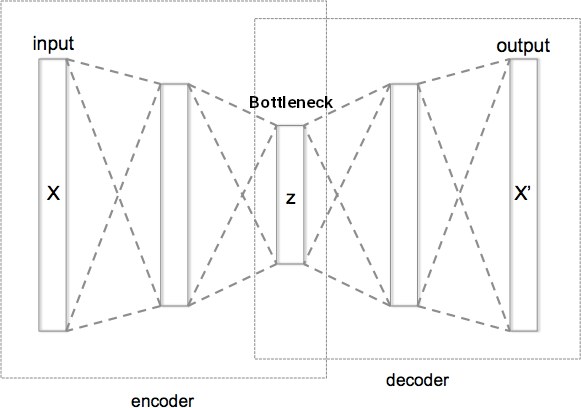
\includegraphics[width=0.75\textwidth]{img/Autoencoder_structure.png}}
    \caption[Autoencoder Structure]{Schematic structure of an autoencoder \cite{autoencoder.pic}, the code element $z$ can be also referred to as latent space.}
    \label{fig:autoencoder}
\end{figure}

A typical autoencoder learns the following mapping while trying to minimize the error (usually the \acrfull{mse}) between its input and output:
\begin{equation}
    X' = D(E(X)) = D(z),~z = E(X)
\end{equation}
Where $D$ is the decoder \emph{forward} pass and $E$ is the encoder one.

\subsubsection{Autoencoders for anomaly detection in images}
An autoencoder learns how to reproduce the data seen during training. This comes in handy when applied to image anomaly detection tasks.
\\
\\
If an autoencoder is trained using only \emph{non-anomalous} images, it learns to reconstruct them with no significant error. However, if an \emph{anomalous} frame would be given as input to the model, it will not reconstruct the anomalies inside the image. Thus returning as output a new image with the anomalous part omitted. The autoencoders we use in this work are strongly limited by their bottleneck. This induces some reconstruction error even in normal samples.

By performing the difference between the input and output image, it is possible to compute an error map~(\autoref{fig:autoencoder-anomaly}). In the Figure, we notice that the autoencoder can correctly reconstruct the scene. However, it was not able to reconstruct the human (anomaly) in the picture. By using the error map shown in the figure it is possible to compute an anomaly score which can be used to determine whether or not a given frame is \emph{anomalous}.

\begin{figure}[!htbp]
    \centering
    \centerline{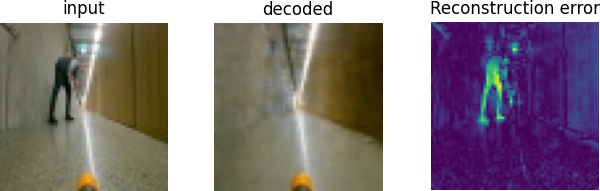
\includegraphics[width=0.9\textwidth]{img/anomaly_det_ex.png}}
    \caption[Autoencoer for anomaly detection]{Example of autoencoder for anomaly detection applied to our collected dataset. The model has been trained only in empty corridors. The human in the input image is thus an anomaly. From left to right: Input image of the model, Output of the model, Error map computed as $error = |input - output|$.}
    \label{fig:autoencoder-anomaly}
\end{figure}


\section{Active Learning}

     \acrfull{al}~\cite{settles.tr09} is a branch of \acrfull{ml} and Human-in-the-loop computing. Its goal is to find and query the best samples (i.e., the most \emph{informative} to a \acrfull{dl} model) to be labeled from an unlabeled pool of data.
    \\
    \\
    \acrshort{dl} has become the state-of-the-art technique for many tasks. However, it relies on an enormous amount of data that needs to be labeled. In some contexts such as medical images, robotics, and safety-critical situations, the need for an expert makes the data labeling expensive, thus limiting the availability of large labeled datasets.
    
    \acrshort{al} overcomes this problem by querying from the unlabeled pool of data the best samples to be labeled using some criteria. The goal is to obtain optimal model performance.
    This approach can drastically reduce labeling costs by reaching near state-of-the-art performance with a fraction of the data used.
    
    Assuming a small labeled dataset $L$, a large pool of unlabeled data $U$, and a group of one or more experts (i.e., persons who label the data) are available. The goal of \acrshort{al} is to find a best $L^*\subseteq L$ given a current \acrshort{dl} model $f(x|L^{\text{'}}),$ $L^{\text{'}}\subseteq L$ where $L^{\text{'}}$ is an intermediate labeled dataset and $U$ is the unlabeled pool from which query new samples for labeling to be added to $L^*$.
    
    It is theorized~\cite{budd2021survey} that it exists some $L^*\subseteq L$ which performance is close to the whole dataset $L$: ($f(x|L^*)\approx f(x|L)$), meaning that a \acrshort{dl} model trained on $L^*$ should achieve similar or equal performance to a model trained on the entire $L$ dataset.
    
    % Assuming a large pool of unlabeled data $U$ is available and a group of one or more oracles (i.e., persons who label the data) is available to label any data on request to be added to the labeled dataset $L$. The goal is to find a best $L^*\subseteq L$ given a current model $f(x|L^{\text{'}}),$ $L^{\text{'}}\subseteq L$ where $L^{\text{'}}$ is an intermediate labeled dataset and $U$ is the unlabeled pool from which to add new data.
    
    % It is theorized \cite{budd2021survey} that exists some $L^*\subseteq L$ which performance is close to the whole dataset $L$: ($f(x|L^*)\approx f(x|L)$), meaning that a model trained on $L^*$ should achieve similar or equal performance to a model trained on the entire $L$ dataset.
    
    One crucial aspect of \acrshort{al} is the query approach. An \acrshort{al} framework queries the samples from the unlabeled set by using some criteria. These chosen samples are then labeled by one or more experts and used to extend the model's knowledge. This can be done in two ways: by fine-tuning the existing model or by retraining it using all the available data.
    Fine-tuning has been demonstrated to outperform a network trained from scratch in the biomedical image field \cite{tajbakhsh2016convolutional}. However, we will test only model retraining in our work.
    
    This section will discuss and introduce some query approaches and several metrics for Active Learning.

    
\subsection{Query approaches}
    
    % A typical \acrshort{al} framework, has to label the most informative samples and use this new data to improve the model.
    Query approaches are used to sample the to-be-labeled data from the \emph{unlabeled} data pool. In the following subsections, we describe some of the query approaches from the literature.
    \\
    \\
    To develop an AL framework the first choice to consider is the type of query. Three choices are available:
    \begin{itemize}
        \item \emph{Stream-based Selective Sampling};
        \item \emph{Membership Query Synthesis};
        \item \emph{Pool-based Sampling}.
    \end{itemize}
    
    \subsubsection*{Stream-based Selective Sampling}
    Stream-based Selective Sampling assumes data is coming in as a continuous stream. The model has to compute an \emph{informativeness} score for each data point and decide whether or not to ask the oracle for annotations.
    Since the decisions are isolated this method does not provide significant benefits when compared to a random decision model.
    
    
    \subsubsection*{Membership Query Synthesis}
    Membership Query Synthesis assumes that the to-be-labeled data is generated instead of being drawn from a real-world data pool.
    The data is generated to be the most \emph{informative} to the model as possible. The generated data is going to be labeled by the oracle and integrated into the training set $L$.
    This approach can be very efficient in finite domains. However, it has some major drawbacks:
    \begin{enumerate}
        \item the model may not know certain unseen areas of the original distribution;
        \item due to some small initial training set, it could also generate data that makes no sense to a human and require annotations for them.
    \end{enumerate}
    
    The recent advance of \emph{Generative Adversarial Networks} (\acrshort{gan}s)~\cite{goodfellow2020generative} has shown great promise for these methods~\cite{budd2021survey}. \acrshort{gan}s can mimic real-world data with high accuracy, making them ideal for this setup.
    
    
    \subsubsection*{Pool-based Sampling}
    Pool-based Sampling assumes a large unlabeled real-world dataset is available. It selects a batch of \textit{N} samples to request labels for.
    This kind of method usually makes use of the currently trained model to make predictions on the unlabeled data to measure the informativeness metric and query the best \textit{N} samples.
    Pool-based methods can be computationally expensive but are the most promising when combined with DL in a deep active learning framework~\cite{budd2021survey}.
    
    
    We chose to work only on \emph{Pool-based sampling} because we have access to the entire data available beforehand, making the stream-based methods not useful.
    On the other hand, we chose not to use membership query synthesis methods for time constraints since they require using and training \acrfull{gan}~\cite{goodfellow2020generative} models.

    
    
    \subsection{Informativeness metrics}
    
    After selecting the query method, an \emph{informativeness} metric has to be defined to select the samples to label.
    Budd et al~\cite{budd2021survey} explain the following types of metrics:
    
    \begin{itemize}
        \item Uncertainty
        \item Representativeness
        \item Generative adversarial networks for informativeness
        \item Learning active learning
    \end{itemize}
    
    For simplicity and time constraints we chose to work only with \emph{uncertainty} and \emph{representativess} metrics. \autoref{tab:AL-SotA-final} summarizes the metrics shown in the next subsections.
    
    % Please add the following required packages to your document preamble:
    % \usepackage{graphicx}
    \begin{table}[ht]
    \centering
    \resizebox{\textwidth}{!}{%
    \begin{tabular}{|c|l|l|l|l|l|}
    \hline
    \textbf{Paper} &
      \multicolumn{1}{c|}{\textbf{Task}} &
      \multicolumn{1}{c|}{\textbf{\begin{tabular}[c]{@{}c@{}}Type of\\ data\end{tabular}}} &
      \multicolumn{1}{c|}{\textbf{\begin{tabular}[c]{@{}c@{}}Uncertainty\\ estimation\end{tabular}}} &
      \multicolumn{1}{c|}{\textbf{\begin{tabular}[c]{@{}c@{}}Uncertainty\\ metrics\end{tabular}}} &
      \multicolumn{1}{c|}{\textbf{\begin{tabular}[c]{@{}c@{}}Representativeness\\ metrics\end{tabular}}} \\ \hline
    \textbf{Wang et al~\cite{wang2016cost}} &
      Classification &
      Images &
       &
      \begin{tabular}[c]{@{}l@{}}\acrshort{lc} Rank,\\ \acrshort{lc} Rank,\\ \acrshort{en} Rank\end{tabular} &
       \\ \hline
    \textbf{Beluch et al~\cite{beluch2018power}} &
      Classification &
      Images &
      \begin{tabular}[c]{@{}l@{}}\acrshort{mc} Dropout,\\ Deep Ensembles.\end{tabular} &
      \begin{tabular}[c]{@{}l@{}}Entropy,\\ \acrshort{bald},\\ Variance\end{tabular} &
      \begin{tabular}[c]{@{}l@{}}Core-set,\\ REPR\end{tabular} \\ \hline
    \textbf{Kirsch et al~\cite{kirsch2019batchbald}} &
      Classification &
      Images &
       &
      Batch\acrshort{bald} &
       \\ \hline
    \textbf{Smailagic et al~\cite{smailagic2018medal}} &
      Classification &
      \begin{tabular}[c]{@{}l@{}}Images\\ (Medical)\end{tabular} &
       &
      \begin{tabular}[c]{@{}l@{}}Distance between output\\ of intermediate \acrshort{cnn} layer\end{tabular} &
      \begin{tabular}[c]{@{}l@{}}Distance between output\\ of intermediate \acrshort{cnn} layer\end{tabular} \\ \hline
    \textbf{Gal et al~\cite{gal2016dropout}} &
      \begin{tabular}[c]{@{}l@{}}Classification,\\ Regression\end{tabular} &
      \begin{tabular}[c]{@{}l@{}}Images,\\ Time series\end{tabular} &
      MC-Dropout &
      \begin{tabular}[c]{@{}l@{}}Bayesian approximation,\\ Gaussian process\end{tabular} &
       \\ \hline
    \textbf{Wen et al~\cite{wen2018comparison}} &
      \begin{tabular}[c]{@{}l@{}}Classification\\ (Binary)\end{tabular} &
      \begin{tabular}[c]{@{}l@{}}Images\\ (Medical)\end{tabular} &
       & {Model posterior based}
       &
       \\ \hline
    \textbf{Yang et al~\cite{yang2017suggestive}} &
      Segmentation &
      \begin{tabular}[c]{@{}l@{}}Images\\ (Biomedical)\end{tabular} &
      Bootstrapping &
      Bootstrapping &
      Cosine similarity \\ \hline
    \textbf{Ozdemir er al~\cite{ozdemir2018active}} &
      Segmentation &
      \begin{tabular}[c]{@{}l@{}}Images\\ (2D, 3D,\\ Medical)\end{tabular} &
      MC-Dropout &
      Borda count &
      \begin{tabular}[c]{@{}l@{}}Cosine similarity,\\ Entropy of intermediate\\ \acrshort{cnn} layer\end{tabular} \\ \hline
    \textbf{Konyushkova et al~\cite{konyushkova2019geometry}} &
      \begin{tabular}[c]{@{}l@{}}Segmentation\\ (Multi-class)\end{tabular} &
      \begin{tabular}[c]{@{}l@{}}Images\\ (2D, 3D,\\ Medical)\end{tabular} &
       &
      \begin{tabular}[c]{@{}l@{}}Entropy:\\     - Shannon,\\     - Selection,\\     - Conditional\\ Geometric entropy\end{tabular} &
       \\ \hline
    \textbf{Sourati et al~\cite{sourati2018active}} &
      \begin{tabular}[c]{@{}l@{}}Segmentation\\ (Semantic)\end{tabular} &
      \begin{tabular}[c]{@{}l@{}}Images\\ (Medical)\end{tabular} &
       &
      Fisher information &
      Fisher information \\ \hline
    \end{tabular}%
    }
    \caption[Metrics for Active Learning]{Different metrics found in the literature for active learning approaches}
    \label{tab:AL-SotA-final}
    \end{table}
    
    \subsubsection*{Uncertainty}
    Uncertainty can be a useful informativeness metric because it is argued that the more uncertain a model prediction is, the more information can be gained by including that sample in the training set.
    
    \paragraph{Uncertainty estimation}
    Uncertainty can be estimated instead of calculated. In the literature, for the context of biomedical images, different methods for estimating uncertainty are proposed.
    
    Monte Carlo Dropout (MC Dropout)~\cite{beluch2018power, gal2016dropout, ozdemir2018active} is one of these. Proposed by Gal et al~\cite{gal2016dropout}, it makes use of regular dropout and interprets it as a Bayesian approximation of the Gaussian Model, a well-known probabilistic model.
    This approach applies dropout during model inference to generate $T$ predictions for each input sample, which can then be averaged or their distribution can be analyzed, estimating the model uncertainty.
    
    % \begin{equation}
    %     p(y=c\mid c, D_{train})=\frac{1}{T}\sum_{t=1}^Tp(y=c\mid x, \omega_t)
    %     \label{eq:mc-dropout}
    % \end{equation}
    
    In addition to \acrshort{mc} Dropout, Beluch et al~\cite{beluch2018power} propose the use of \emph{Deep Ensembles} to estimate model uncertainty. This approach trains $N$ classifiers and then computes the average softmax output of the $N$ predictions for each unlabeled sample.
    
   Yang et al~\cite{yang2017suggestive} make use \emph{bootstrapping} \cite{efron1994introduction} to estimate the model uncertainty. This method works by training a set of models on a different restricted random subset (random sampling with replacement) of the training data. The method then computes the variance between the model predictions.
    
    \paragraph{Uncertainty metrics}
    Uncertainty can be computed in several ways, depending on the task and field of the problem.
    It is usually computed using the lowest class probabilities, marginal sampling, or entropy \cite{shannon1948mathematical}.
    
    Other uncertainty methods have been proposed, such as \acrfull{ceal}~\cite{wang2016cost}.
    % \begin{dmath}
    %     \min_{W, y_i, i\in U} -\frac{1}{n}\sum_{i=1}^n\sum_{j=1}^m\mathbf{1}\{y_i=j\}\log p(y_i=j\mid x_i;W)
    %     \label{eq:ceal}
    % \end{dmath}
    It uses traditional \acrshort{al} entropy-based methods to generate the $D_L$ dataset with the most uncertain samples. It then introduces an additional step in which the most confident samples (whose \emph{entropy} is below a threshold $\omega$) are added to $D_H$. Both $D_L$ and $D_H$ are then used to fine-tune the model for a given number of iterations. Then the threshold $\omega$ is updated and the samples from $D_H$ are added back to the unlabeled dataset.
    This method showed state-of-the-art performance using less than 60\% of the available data~\cite{wang2016cost}.
    
    % Other methods, referred to as \textit{Query by consensus} are used in conjunction with ensembling.
    
    Another approach uses Bayesian \acrshort{cnn}s for AL in a method named \acrfull{bald} \cite{gal2017deep}.
    This approach is based on a Bayesian \acrshort{cnn}. It produces a set of predictions using all the parameters and a set of stochastic predictions for each sample in the unlabeled dataset. Then the \acrshort{bald} acquisition function~\cite{houlsby2011bayesian} is calculated as the difference in entropy between the average prediction and the average stochastic prediction.
    % \begin{dmath}
    %     {\mathbb{I}[y, \omega \mid \mathbf{x}, \mathcal{D}_{train}] := \mathbb{H}[y\mid\mathbf{x}, \mathcal{D}_{train}] - \mathbb{E}_{p(\omega\mid \mathcal{D}_{train})}\left[\mathbb{H}[y\mid\mathbf{x}, \omega]\right]} = {-\sum_{c}p(y=c\mid\mathbf{x}, \mathcal{D}_{train})\log p(y=c\mid\mathbf{x}, \mathcal{D}_{train})} + {\mathbb{E}_{p(\omega\mid\mathcal{D}_{train})}\left[\sum_c p(y=c\mid\mathbf{x}, \omega)\log p(y=c\mid\mathbf{x}, \omega)\right]}
    %     \label{eq:bald}
    % \end{dmath}
    This method has been shown effective for \acrshort{al}~\cite{gal2016dropout}. However, it can result in redundant and very similar unlabeled samples being chosen. Batch\acrshort{bald}~\cite{kirsch2019batchbald} solves this issue by calculating the mutual information in batches instead of on all the datasets. 
    
    % For binary classification tasks \cite{wen2018comparison} proposes the following uncertainty metric (\autoref{eq:unc}):
    % \begin{dmath}
    %     {unc = -\mid p_i - 0.5\mid},\\
    %     {p_i=P\{f(x_i) = 1\} \in \left[0,1\right]}
    %     \label{eq:unc}
    % \end{dmath}
    % Where $p_i$ is the posterior probability, $f$ is the trained model. The most uncertain samples will be the ones with posterior probability $x_i$ close to 0.5.
    
    In the field of medical image segmentation, Konyushkova et al~\cite{konyushkova2019geometry} propose a novel uncertainty metric that considers the geometrical properties of the images.
    The proposed method builds a graph from the image. Each segmented region (i.e., \emph{superpixel}) becomes a node, with edges linking neighbor regions. Edges in the graph are weighted with the probability of the transition to the same label as a neighbor. The intuition behind this metric is that the closer two regions are, the more likely they are to have the same label \cite{konyushkova2019geometry}.
    

% \begin{figure}[!htb]
%     \centering
%     \centerline{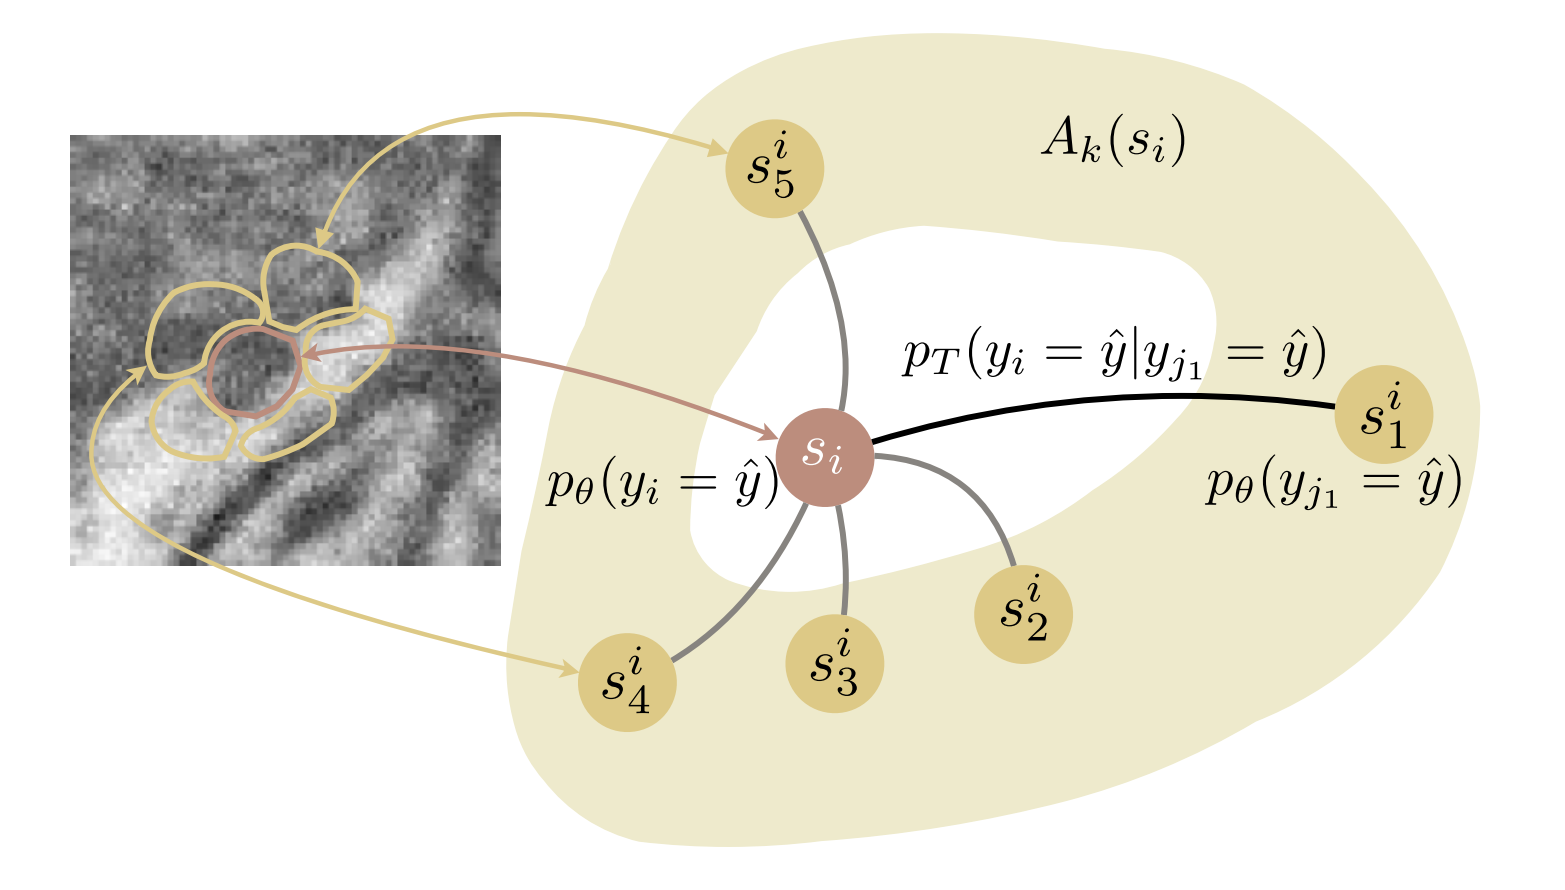
\includegraphics[width=0.9\textwidth]{img/geom_uncert.png}}
%     \caption[Autoencoder Structure]{\cite{konyushkova2019geometry} Graph representation of image on the left. $A_k(i)$ is the \emph{neighborhood} of node $s_i$, $p_T$ is the probability for node $s_i$ of having the same probability of a node $s^i_j$, and $p_{\theta}(y_i=\hat{y} \mid \mathbf{x}_i)$ is the probability that the class of $s_i$ ($y_i$) is $\hat{y}$, given only the feature vector $\mathbf{x}_i$.}
%     \label{fig:geom-unc}
% \end{figure}

% \begin{dmath}
%     {p_G^{\tau + 1}(y_i = \hat{y}) = \sum_{s_j \in A_k(s_i)}p_T(y_i=\hat{y}|p_G^{\tau}(y_j=\hat{y})}, \\
%     p_G^0(y_i = \hat{y})=p_{\theta }(y_j=\hat{y}|x_j)
%     \label{eq:geom-unc}
% \end{dmath}
    
    \subsubsection*{Representativeness}
    The representativeness metric is used to avoid problems that arise by focusing only on uncertainty to select the next samples to label (i.e., focusing on small regions of the distribution and redundancy/similarity in chosen data).
    
    Representativeness metrics used are usually based on some distance metric between samples.
    
    % \begin{equation}
    %     u = \argmax_{i\in [n]\textbackslash s}~\min_{j\in s}~dist(x_i, x_j)
    %     \label{eq:core-set}
    % \end{equation}
    Beluch et al~\cite{beluch2018power} uses \emph{core-set} and \emph{REPR} methods as \emph{representativeness} metrics.
    The First method is a core-set-approach~\cite{sener2017geometric} that chooses $p$ points that minimize the maximum distance between the point $x_i$ and its closest neighbor $x_j$ in the chosen subset $s$. This approach combines both uncertainty and representativeness ideas in a single metric; the resulting metric $u$ is computed greedily.

    The REPR method on the other hand chooses points that best represent the rest of the data distribution greedily.
    Each sample of the unlabeled dataset $U$ has a computed \emph{representativeness} score, defined as the similarity between this point and its most similar one in the labeled set $L$. 
    This approach encourages $L$ to be as diverse as possible to represent in the best way the distribution of the unlabeled data. The similarity function Beluch et al~\cite{beluch2018power} use is the Euclidean norm.
    
    % \begin{dmath}
    %     {R(L, U) = \sum_{x_j \in U}r(L, x_j)}
    %     {r(L, x_j) = \max_{x_i \in L}~sim(x_i, x_j)}
    %     \label{eq:REPR}
    % \end{dmath}
    
    Samilagic et al~\cite{smailagic2018medal} propose a novel model and a new metric. They try to combine uncertainty and representativeness by measuring the distance between the outputs of internal layers of a \acrshort{cnn}. They test different distance metrics, with the Euclidean distance performing the best.
    
    % \begin{dmath}
    %     {s(x) = \frac{1}{N}\sum_{i=1}^Nd(f(x_i), f(x)),}
    %     \\
    %     {x_i\in D_{train}}
    %     \label{eq:intermediate-cnn}
    % \end{dmath}
    
    
    Ozdemir et al~\cite{ozdemir2018active} take the work done by Smailagic et al~\cite{smailagic2018medal} and try to improve it by letting the model learn representativeness by maximizing the activation entropy loss, a novel form of regularization.
    
    % \begin{equation}
    %     L_{ent} = -\sum_{x}\mathbb{H}(R^{l_{abst}, x})
    %     \label{eq:entropy_loss}
    % \end{equation}
    
    \subsubsection*{Generative adversarial networks for informativeness}
    \acrshort{gan}s can be used in an active learning framework to generate new data to be labeled and a metric of informativeness could be returned by the generator and/or the discriminator models~\cite{ravanbakhsh2020human, mahapatra2018efficient, budd2021survey}.
    
    A \acrshort{gan} is a neural network proposed by Goodfellow et al~\cite{goodfellow2020generative}. It is composed of two networks: a \emph{generator} and a \emph{discriminator}.
    
    The two networks are set up in an adversarial manner: the objective of the generator is to generate samples that will fool the discriminator. The discriminator, on the other hand, has to predict whether the input sample was real or generated.
    
    Both networks are trained at the same time, in a \emph{minmax} setup: each network minimizes its loss and tries to maximize the loss of the other.
    
    \subsubsection*{Learning active learning}
    The methods discussed so far rely on defined heuristics. The goal of \textit{Learning active learning} techniques is to use a model to infer the best selection strategy based on the experience of previous AL outcomes. These techniques are an ideal use case for reinforcement learning (LR) methods~\cite{budd2021survey}.
    A data selection policy learned this way can be agnostic to the data selection strategies, potentially achieving better results and reaching state-of-the-art performance with even less sample than the heuristics shown above.
    
% \subsection{Interactive Refinement}
%     After the model training phase, the role of oracles can still be useful to improve the model performance and generalization of unseen data. This approach is named \textit{Interactive Refinement}. The basic idea behind this approach is to apply a similar concept of \acrshort{al} to a production-ready model to improve its generalization on slightly different tasks.

